\documentclass{standalone}
\usepackage[mh]{mikoslides}
% this file defines root path local repository
\defpath{MathHub}{/Users/kohlhase/localmh/MathHub}
\mhcurrentrepos{MiKoMH/talks}
\libinput{WApersons}
% we also set the base URI for the LaTeXML transformation
\baseURI[\MathHub{}]{https://mathhub.info/MiKoMH/talks}

\usetikzlibrary{backgrounds,shapes,fit,shadows}
%\libinput{preamble}
\begin{document}
    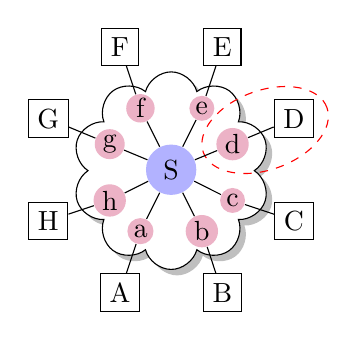
\begin{tikzpicture}[scale=1.3]
      \tikzstyle{withshadow}=[draw,drop shadow={opacity=.5},fill=white]
      \tikzstyle{system}=[draw]
      \tikzstyle{standard}=[circle,fill=blue!30]
      \tikzstyle{interface}=[circle,fill=purple!30,inner sep = 1pt,]
      \node[system] (a) at (0,.3) {A};
      \node[system] (b) at (1,.3) {B};
      \node[system] (c) at (1.7,1) {C};
      \node[system] (d) at (1.7,2) {D};
      \node[system] (e) at (1,2.7) {E};
      \node[system] (f) at (0,2.7) {F};
      \node[system] (g) at (-.7,2) {G};
      \node[system] (h) at (-.7,1) {H};
      \node[standard] (m) at (.5,1.5) {S};
      \node[interface] (ia) at (0.2,.9) {a};
      \node[interface] (ib) at (.8,.9) {b};
      \node[interface] (ic) at (1.1,1.2) {c};
      \node[interface] (id) at (1.1,1.75) {d};
      \node[interface] (ie) at (.8,2.1) {e};
      \node[interface] (if) at (0.2,2.1) {f};
      \node[interface] (ig) at (-.1,1.75) {g};
      \node[interface] (ih) at (-.1,1.2) {h};
      \draw (m) -- (ia) -- (a);
      \draw (m) -- (ib) -- (b);
      \draw (m) -- (ic) -- (c);
      \draw (m) -- (id) -- (d);
      \draw (m) -- (ie) -- (e);
      \draw (m) -- (if) -- (f);
      \draw (m) -- (ig) -- (g);
      \draw (m) -- (ih) -- (h);
      \begin{pgfonlayer}{background}
        \node[draw,cloud,fit=(ia) (ib) (ic) (id) (ie) (if) (ig) (ih),
                   inner sep=-7pt,withshadow] (st) {};
        \node[fit=(d) (id),ellipse,inner sep=-1pt,rotate=20,draw,dashed,red] (sys) {};
      \end{pgfonlayer}
      \end{tikzpicture}
\end{document}
%%% Local Variables: 
%%% mode: latex
%%% TeX-master: t
%%% End: 
